\documentclass[mathserif]{beamer}
\usepackage{epstopdf}
\usepackage{amsmath}
\usepackage{helvet}
\usepackage{listings}
\usepackage{algorithm2e}
\usetheme{CambridgeUS}
%\usecolortheme{whale}


\title[Beamer themes] % (optional, only for long titles)
{\textbf{This is just a text with beamer presentations because I want other theme colors}}
\subtitle{We want more colors}
\author{David Anchieta}
\subject{\LaTeX}

\begin{document}
	\frame{\titlepage}

	\section*{Outline}
	\begin{frame}{Outline}		
		\tableofcontents
	\end{frame}
	
	%========================================================================
	%FIRST SECTION STARTS HERE
	%========================================================================
	\section{Single tone case}
	\begin{frame}{Estimating frequency and amplitude of a single tone}
		Given a complex sinusoid defined by:
		\begin{equation*}
			r(t) = A_{1}e^{j2\pi f_1 t} + z(t)
		\end{equation*}
		Where $z(t)$ is a complex Gaussian white noise with zero mean and variance $\sigma^2$.
		
		Givens a set of samples from $r(t)$, how could we estimate the values of $A_1$ and $f_1$?	
		
	\end{frame}
	
	
	\subsection{Maximum likelihood estimators of frequency and amplitude}
	
	\begin{frame}{Note on Maximum Likelihood Estimation \#1}
		\begin{itemize}
			\item It's a method to estimate parameters of a statistical model.
			\item The value of the Maximum Likelihood Estimator of a parameter must make the observed data more likely.
		\end{itemize}
		\pause
		An example of maximum likelihood estimator: The sample mean of a set of $n$ observations from a random variable $X$.
		\begin{gather*}
			M_n = \frac{1}{n}\sum_{i=1}^nX_i\\
			\only<3->{ \lim_{n \to \infty}M_n = \mathrm{E}\{X\}}
		\end{gather*}
	\end{frame}
	
	\begin{frame}{Estimating frequency and amplitude of a single tone}
		\begin{figure}
			\centering
			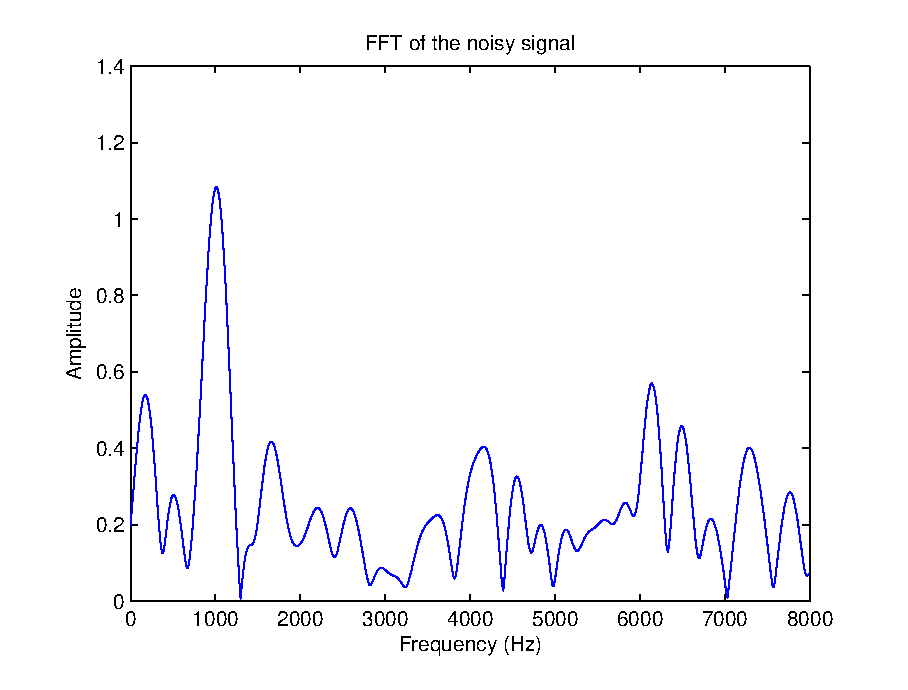
\includegraphics[scale=0.375]{./img3/singleTonewoMHFig2.eps}
			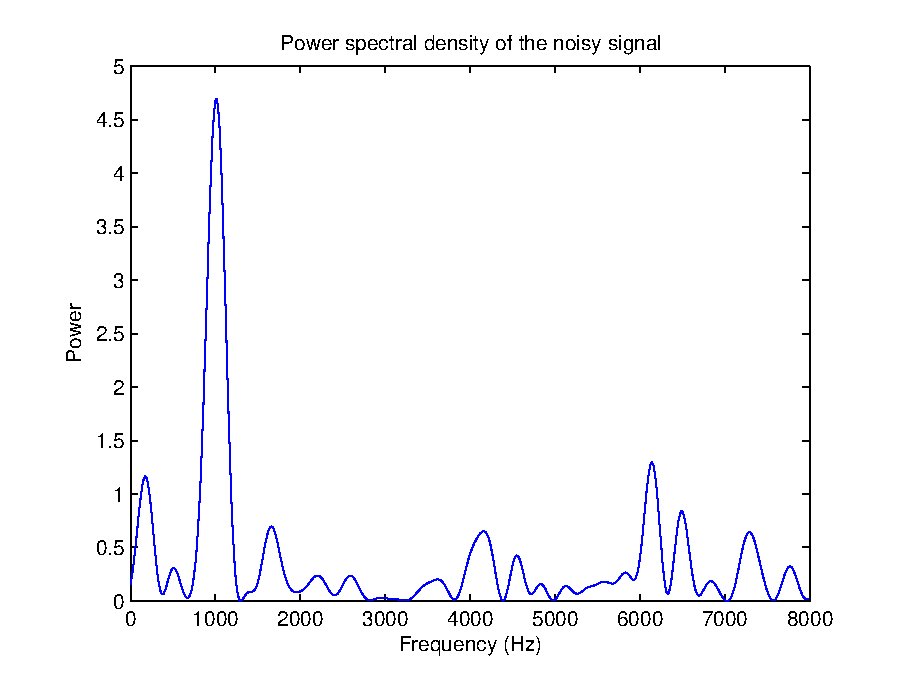
\includegraphics[scale=0.375]{./img3/singleTonewoMHFig3.eps}
			\caption{Discrete-time Fourier Transform and power spectral density of the signal with added noise.}
		\end{figure}
	\end{frame}
	
	%========================================================================
	%I START TO TALK ABOUT PDF'S HERE
	%========================================================================
	\subsection{Computing probability density functions}
	\begin{frame}{Defining the PDF of the frequency}
		Being $N$ the number of samples and $T_s$ the sampling period $1/f_s$, we have.
		\begin{gather*}
			\mathbf{r} =  [r(0) \; \; r(T_s) \; \; r(2T_s) \; \dots \; r((N-1)T_s)]^T \\
			\mathbf{e_1} =  [e^{j2\pi f_10} \; e^{j2\pi f_1T_s} \; \dots \; e^{j2\pi f_1(N-1)T_s}]^T \\		
			\mathbf{r} = A_1\mathbf{e_1} + \mathbf{n} \\
			\mathrm{p}(\mathbf{r}|f_1,A_1) = \frac{1}{\pi^N\sigma^{2N}}\exp\left[-\frac{(\mathbf{r}-A_1\mathbf{e_1})'
				(\mathbf{r}-A_1\mathbf{e_1})}{\sigma^2}\right] \\
			\mathrm{p}(\mathbf{r}|A_1) = \int \mathrm{p}(\mathbf{r}|f_1,A_1)\mathrm{p}(f_1)df_1\\
			\mathrm{p}(f_1|\mathbf{r},A_1) = \frac{\mathrm{p}(\mathbf{r}|f_1,A_1)\mathrm{p}(f_1)}{\mathrm{p}(\mathbf{r}|A_1)} \\
		\end{gather*}
	\end{frame}
	
	\begin{frame}{Defining the PDF of the frequency}
		\begin{figure}
			\centering
			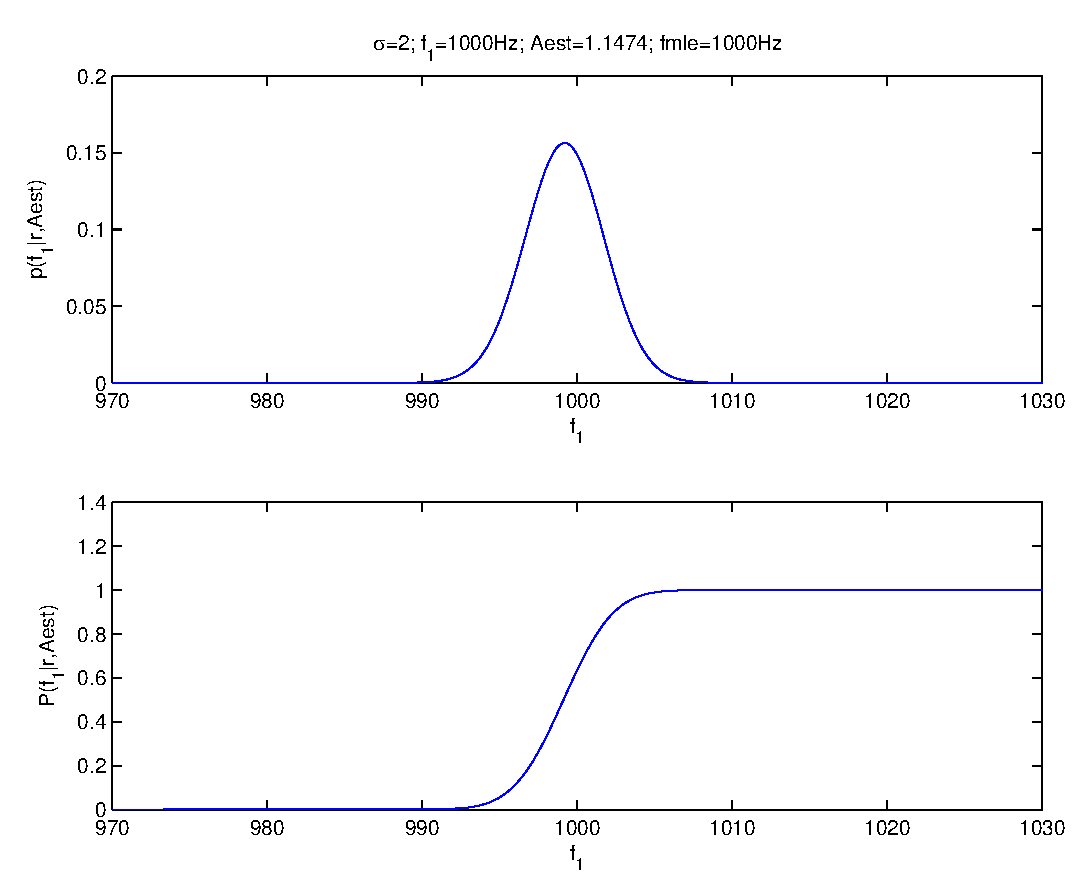
\includegraphics[scale=0.345]{./img3/singleTonewoMHFig11.eps}
			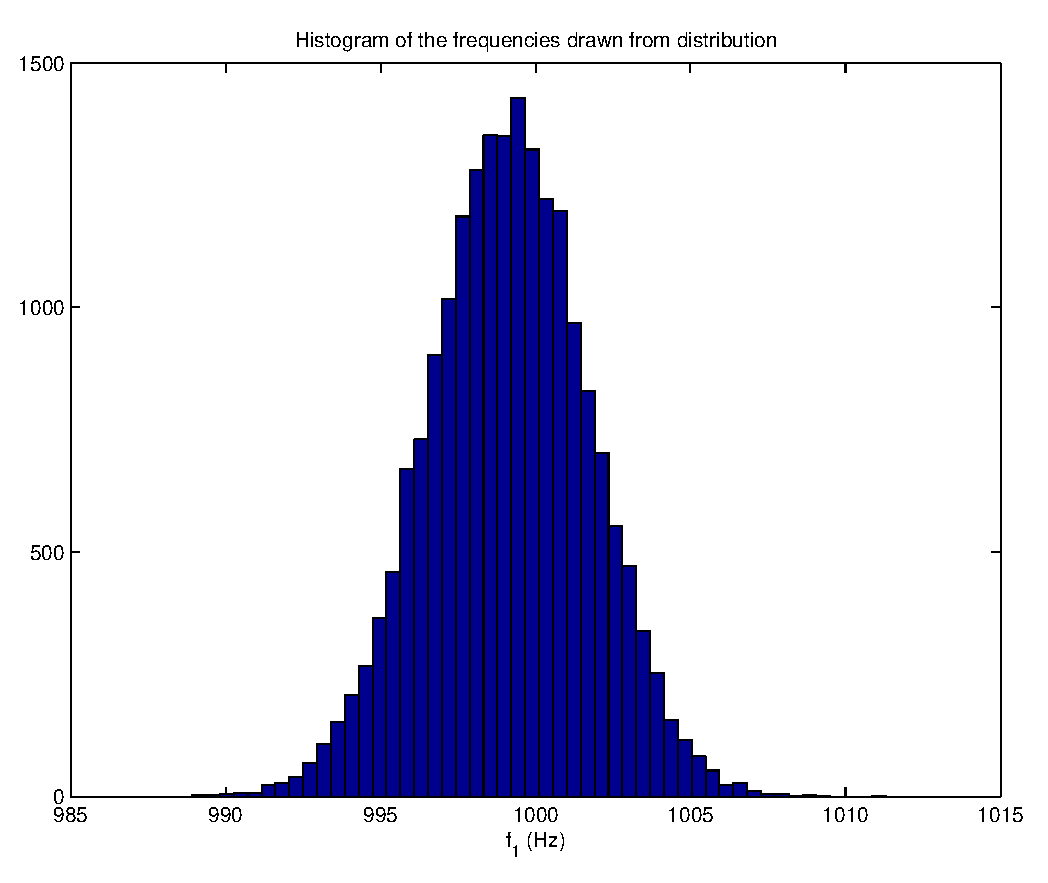
\includegraphics[scale=0.345]{./img3/singleTonewoMHFig12.eps}
			\caption{PDF of the frequency conditioned on the MLE of the amplitude.}
		\end{figure}
	\end{frame}	
	

	
\end{document}